\clearpage
\subsection{Task 3: การพยากรณ์ยอดใช้จ่ายรายเดือนของผู้เล่น (Player Monthly Spending Prediction)}
\label{subsec:task3}

ภารกิจที่ 3 มุ่งเน้นการพยากรณ์ยอดใช้จ่ายรวมในเกมของผู้เล่นแต่ละรายภายใน 30 วันข้างหน้า (\feat{spending\_30d}, หน่วยบาท: THB) บนชุดข้อมูลฝึกสอน 104,000 แถว และชุดข้อมูลทดสอบ 25,889 แถว โดยมีฟีเจอร์ตั้งต้น 32 ตัวแปร แม้จะเป็นโจทย์ถดถอย (Regression) ที่มีสัญญาณเชิงประวัติศาสตร์แข็งแกร่งจากยอดเดือนก่อนหน้า (\feat{prev\_month\_spending}) แต่ความท้าทายเชิงวิศวกรรมที่แท้จริงเกิดจากโครงสร้างข้อมูลแบบกึ่งต่อเนื่องที่มีศูนย์เกือบครึ่งหนึ่ง (Zero-Inflated) การกระจุกตัวของมูลค่าในกลุ่มผู้เล่นระดับสูง (Whales) และการเลือกจุดทำงานที่สอดคล้องกับโครงสร้างทางคณิตศาสตร์ของตัวชี้วัด Normalized Mean Absolute Error (NMAE) อย่างเคร่งครัด

% ----------------------------------------------------------------------
\subsubsection{บริบททางธุรกิจและกลไกของ Metric NMAE}
\label{subsubsec:t3_business_metric}

จากบริบทการดำเนินงานของบริษัท Karena Thailand ความแม่นยำในการพยากรณ์ยอดใช้จ่ายรายบุคคลส่งผลโดยตรงต่อ 4 หน่วยงานหลักในองค์กร ได้แก่
\begin{enumerate}
    \item \textbf{ฝ่ายการเงิน (Finance Forecasting):} การประมาณการรายได้รายไตรมาสของบริษัทคลาดเคลื่อนจากเป้าหมายจริงถึง \textbf{35--40\%} อย่างต่อเนื่อง ทำให้การจัดสรรงบประมาณ แผนการจ้างงาน และความเชื่อมั่นของนักลงทุนขาดฐานข้อมูลเชิงปริมาณรองรับ
    \item \textbf{ทีมดูแลลูกค้า VIP จำนวน 20 คน (VIP Support Triage):} ที่ผ่านมาทีมไม่มีตัวชี้วัดศักยภาพการใช้จ่ายของผู้เล่น จึงทุ่มเทเวลาดูแลผู้เล่นที่เล่นเกมนาน 150 รายซึ่งมียอดใช้จ่ายรวมกันเพียง \textbf{12,000 THB} ขณะที่ผู้เล่นระดับ Whale ซึ่งมียอดใช้จ่าย \textbf{255,000 THB} ต้องรอการตอบกลับ Ticket นานถึง 3 วันและย้ายไปเล่นเกมคู่แข่งในที่สุด
    \item \textbf{ฝ่ายการตลาด (Targeted Promotions):} การส่งโค้ดส่วนลด 50\% แบบสุ่มให้ผู้เล่นจำนวนมากรวมถึงกลุ่ม Whale ที่พร้อมจ่ายเต็มราคาอยู่แล้ว ก่อให้เกิดการสูญเสียรายได้เกินกว่า \textbf{6 ล้านบาทต่อเดือน}
    \item \textbf{ฝ่ายบริหารกิจกรรม (Event Scheduling):} จำเป็นต้องกำหนดเวลาปล่อยคอนเทนต์ใหม่และกิจกรรมจำกัดเวลาให้สอดคล้องกับช่วงที่ผู้เล่นที่พร้อมจ่ายเงินมีพฤติกรรมการใช้งานสูงสุด
\end{enumerate}

สำหรับเกณฑ์ประเมินผลของภารกิจนี้คือ \textbf{NMAE Score} ซึ่งนิยามในรูปแบบความแม่นยำเชิงบวก (ยิ่งสูงยิ่งดี) จากอัตราส่วนความคลาดเคลื่อนสัมบูรณ์รวมต่อยอดใช้จ่ายรวมทั้งหมดในชุดประเมิน:
\begin{equation}
\label{eq:t3_nmae}
\text{NMAE Score} = \frac{1}{1 + \dfrac{\sum_{i=1}^{N} |y_i - \hat{y}_i|}{\sum_{i=1}^{N} y_i}} = \frac{1}{1 + \dfrac{\text{MAE}(\mathbf{y}, \hat{\mathbf{y}})}{\bar{y}}}, \qquad y_i \ge 0
\end{equation}
สมการที่~\eqref{eq:t3_nmae} มีสมบัติสำคัญ 2 ประการต่อการออกแบบโมเดล ประการแรก หากโมเดลทำนายเป็นศูนย์ทั้งหมด ($\hat{y}_i = 0$ ทุกแถว) อัตราส่วนความคลาดเคลื่อนรวม $E / Y = \sum |y_i| / \sum y_i = 1$ จะให้คะแนนพื้นฐาน \textbf{All-Zero Baseline = 0.50000} ประการที่สอง การเพิ่มค่า $\text{NMAE Score}$ ให้สูงสุดสมมูลกับการลดผลรวมความคลาดเคลื่อนสัมบูรณ์ $\sum_{i=1}^N |y_i - \hat{y}_i|$ (L1 / MAE Loss) ให้น้อยที่สุด ซึ่งหมายความว่าความคลาดเคลื่อน 1 บาทจากผู้เล่นระดับ Whale มีน้ำหนักเท่ากับ 1 บาทจากผู้เล่นทั่วไป และเมื่อโมเดลต้องเผชิญกับความไม่แน่นอนแบบ Zero-Inflated คำตอบที่เหมาะสมที่สุดทางคณิตศาสตร์ไม่ใช่ค่าคาดหมาย (Conditional Mean) แต่เป็น \textbf{ค่ามัธยฐานแบบมีเงื่อนไขของส่วนผสม (Conditional Mixture Median)}

\begin{insightbox}[การพิสูจน์ทางคณิตศาสตร์: เหตุใด NMAE จึงบังคับใช้ Conditional Mixture Median]
ให้ตัวแปรสุ่ม $Y \ge 0$ มีการแจกแจงแบบ Hurdle Mixture โดยมีโอกาสที่จะจ่ายเงิน $p = P(Y > 0 \mid \mathbf{x})$ และฟังก์ชันแจกแจงสะสมแบบมีเงื่อนไขเมื่อจ่ายเงินคือ $F_+(y \mid \mathbf{x}) = P(Y \le y \mid Y > 0, \mathbf{x})$ ดังนั้น CDF รวมของ $Y$ เมื่อทราบคุณลักษณะ $\mathbf{x}$ คือ
\[
F(y \mid \mathbf{x}) = (1 - p)\,\mathbb{I}[y \ge 0] + p\,F_+(y \mid \mathbf{x})\,\mathbb{I}[y > 0]
\]
ตัวพยากรณ์ $\hat{y}^*$ ที่ทำให้ความเสี่ยงของ L1 Loss $\mathbb{E}[|Y - \hat{y}| \mid \mathbf{x}]$ มีค่าต่ำสุดคือมัธยฐานที่ตำแหน่งสะสม $0.5$ พอดี ($\inf\{y \ge 0 : F(y \mid \mathbf{x}) \ge 0.5\}$) ซึ่งแยกพิจารณาได้เป็น 2 กรณี:
\begin{enumerate}
    \item \textbf{กรณี $p \le 0.5$:} มวลความน่าจะเป็นที่จุดศูนย์เพียงอย่างเดียวคือ $1 - p \ge 0.5$ ดังนั้นคำตอบที่ลด L1 Loss ได้ดีที่สุดคือ \textbf{$\hat{y}^* = 0$} อย่างแน่นอน
    \item \textbf{กรณี $p > 0.5$:} ต้องสะสมความน่าจะเป็นจากส่วนที่เป็นบวกเพิ่มจนถึงระดับ $0.5$ นั่นคือ
    \begin{equation}
    \label{eq:t3_hurdle_quantile}
    (1 - p) + p \cdot q = 0.5 \implies q = 1 - \frac{1}{2p} \in (0, 0.5]
    \end{equation}
    ดังนั้น $\hat{y}^* = F_+^{-1}\!\left(1 - \dfrac{1}{2p} \;\middle|\; \mathbf{x}\right)$
\end{enumerate}
ข้อสรุปเชิงวิศวกรรมที่ได้จากสมการที่~\eqref{eq:t3_hurdle_quantile} คือ ระดับควอนไทล์ $q$ ที่ใช้จริงจะไม่มีทางเกิน $0.50$ (เมื่อ $p \to 1$ ค่า $q \to 0.50$) โมเดลส่วนปริมาณจึงจำเป็นต้องเรียนรู้เฉพาะควอนไทล์ช่วง $\alpha \in [0.02, 0.50]$ เท่านั้น และการใช้ค่าคาดหมาย $p \cdot \mathbb{E}[Y \mid Y > 0, \mathbf{x}]$ จะให้ผลทำนายที่สูงเกินจริงเมื่อเทียบกับจุดสมดุลของ MAE บนข้อมูลที่เบ้ขวาอย่างรุนแรง
\end{insightbox}

% ----------------------------------------------------------------------
\subsubsection{ข้อค้นพบจาก EDA และโครงสร้างการสร้างข้อมูล}
\label{subsubsec:t3_eda}

การวิเคราะห์ข้อมูลเชิงสำรวจ (EDA) และการแกะรอยกระบวนการสร้างข้อมูล (Data-Generating Process: DGP) ใน \feat{work/insight/c01\_t3\_generator.py} ถึง \feat{c05\_t3\_decomp.py} และ \feat{t3/research/round9\_sonnet/} เผยให้เห็นโครงสร้างหลักของปัญหาในรูปแบบ \textit{Claim $\rightarrow$ Evidence $\rightarrow$ Implication} ดังต่อไปนี้

\paragraph{1. ความไม่สมมาตรแบบ Zero-Inflated และการครอบงำของกลุ่ม Whale}
\textbf{Claim:} ยอดใช้จ่ายมีความเบ้ขวาสุดขั้วร่วมกับฐานศูนย์ขนาดใหญ่ โดยผู้เล่นกลุ่ม Whale (\feat{segment} = 3) แม้จะเป็นส่วนน้อยแต่เป็นผู้กำหนดทั้งรายได้รวมและสัดส่วนความคลาดเคลื่อนหลักของโมเดล \\
\textbf{Evidence:} ในชุดฝึกสอน 104,000 แถว มีผู้ไม่มียอดใช้จ่าย ($y = 0$) สูงถึง \textbf{50,049 แถว (48.12\%)} และมีผู้จ่ายเงิน ($y > 0$) \textbf{53,951 แถว (51.88\%)} ทำให้ค่าเฉลี่ยทั้งชุดอยู่ที่ \textbf{10,497.04 THB} ขณะที่ค่ามัธยฐานอยู่เพียง \textbf{79.44 THB} ส่วนเปอร์เซ็นไทล์ที่ 99 (\feat{p99}) สูงถึง \textbf{150,032.30 THB} และมีเพดานตัดยอดสูงสุด (Hard Cap) ที่ \textbf{300,000.0 THB} (พบ 15 แถวที่แตะเพดาน และค่าบวกต่ำสุดคือ 0.09 THB) เมื่อจำแนกสถิติตาม \feat{segment} ดิบดังแสดงในตารางที่~\ref{tab:t3_segment_breakdown} และรูปที่~\ref{fig:t3_whale_budget}(a) จะพบว่ากลุ่ม Whale (\feat{segment} = 3) มีจำนวน \textbf{14,579 แถว} คิดเป็นเพียง \textbf{14.02\%} ของข้อมูลทั้งหมด (หรือ 14.87\% ของ 98,065 แถวที่ทราบ \feat{segment}) แต่มีอัตราการใช้จ่ายสูงถึง 92.85\% (ศูนย์เพียง 7.15\%) ยอดเฉลี่ย 65,357.70 THB และครองยอดใช้จ่ายรวมถึง \textbf{87.28\%} พร้อมทั้งสร้างความคลาดเคลื่อน OOF สูงถึง \textbf{79.37\%} ของความคลาดเคลื่อนรวมทั้งหมด \\
\textbf{Implication:} การสุ่มแบ่งข้อมูล Cross-Validation แบบธรรมดาอาจทำให้แต่ละ Fold มีสัดส่วนของ Whale หรือหางขวาไม่สมดุล จึงต้องใช้ \feat{StratifiedKFold} ที่แบ่งชั้นตามตัวแปรศูนย์ร่วมกับ 4 Quartiles ของผู้จ่ายเงิน และแนวทางการปรับปรุงโมเดลควรมุ่งลดความผิดพลาดเชิงสัมพัทธ์ในกลุ่ม Whale โดยไม่ทำลายความแม่นยำของ Conditional Quantile

\begin{table}[htbp]
\centering
\caption{การกระจายของข้อมูล ยอดใช้จ่ายรวม และสัดส่วนความคลาดเคลื่อน OOF ของโมเดลสุดท้าย (\protect\feat{bag\_q10p10}) จำแนกตาม \protect\feat{segment} ดิบในชุดฝึกสอน}
\label{tab:t3_segment_breakdown}
\footnotesize
\setlength{\tabcolsep}{4pt}
\begin{tabularx}{\textwidth}{@{}Xrrrrrr@{}}
\toprule
\textbf{กลุ่มผู้เล่น (\feat{segment})} & \textbf{จำนวนแถว} & \textbf{สัดส่วน (\%)} & \textbf{อัตรา $y=0$ (\%)} & \textbf{เฉลี่ย $y$ (THB)} & \textbf{สัดส่วนยอด (\%)} & \textbf{สัดส่วน OOF $|e|$ (\%)} \\
\midrule
Casual (\feat{0}) & 39,241 & 37.73 & 72.44 & 73.96 & 0.27 & 1.02 \\
Grinder (\feat{1}) & 24,483 & 23.54 & 47.96 & 944.37 & 2.12 & 5.97 \\
Social (\feat{2}) & 19,762 & 19.00 & 30.65 & 2,283.85 & 4.13 & 7.68 \\
\textbf{Whale (\feat{3})} & \textbf{14,579} & \textbf{14.02} & \textbf{7.15} & \textbf{65,357.70} & \textbf{87.28} & \textbf{79.37} \\
ไม่ทราบกลุ่ม (\feat{NaN}) & 5,935 & 5.71 & 46.84 & 11,404.51 & 6.20 & 5.96 \\
\midrule
\textbf{รวมทั้งหมด} & \textbf{104,000} & \textbf{100.00} & \textbf{48.12} & \textbf{10,497.04} & \textbf{100.00} & \textbf{100.00} \\
\bottomrule
\end{tabularx}
\end{table}

\begin{figure}[htbp]
    \centering
    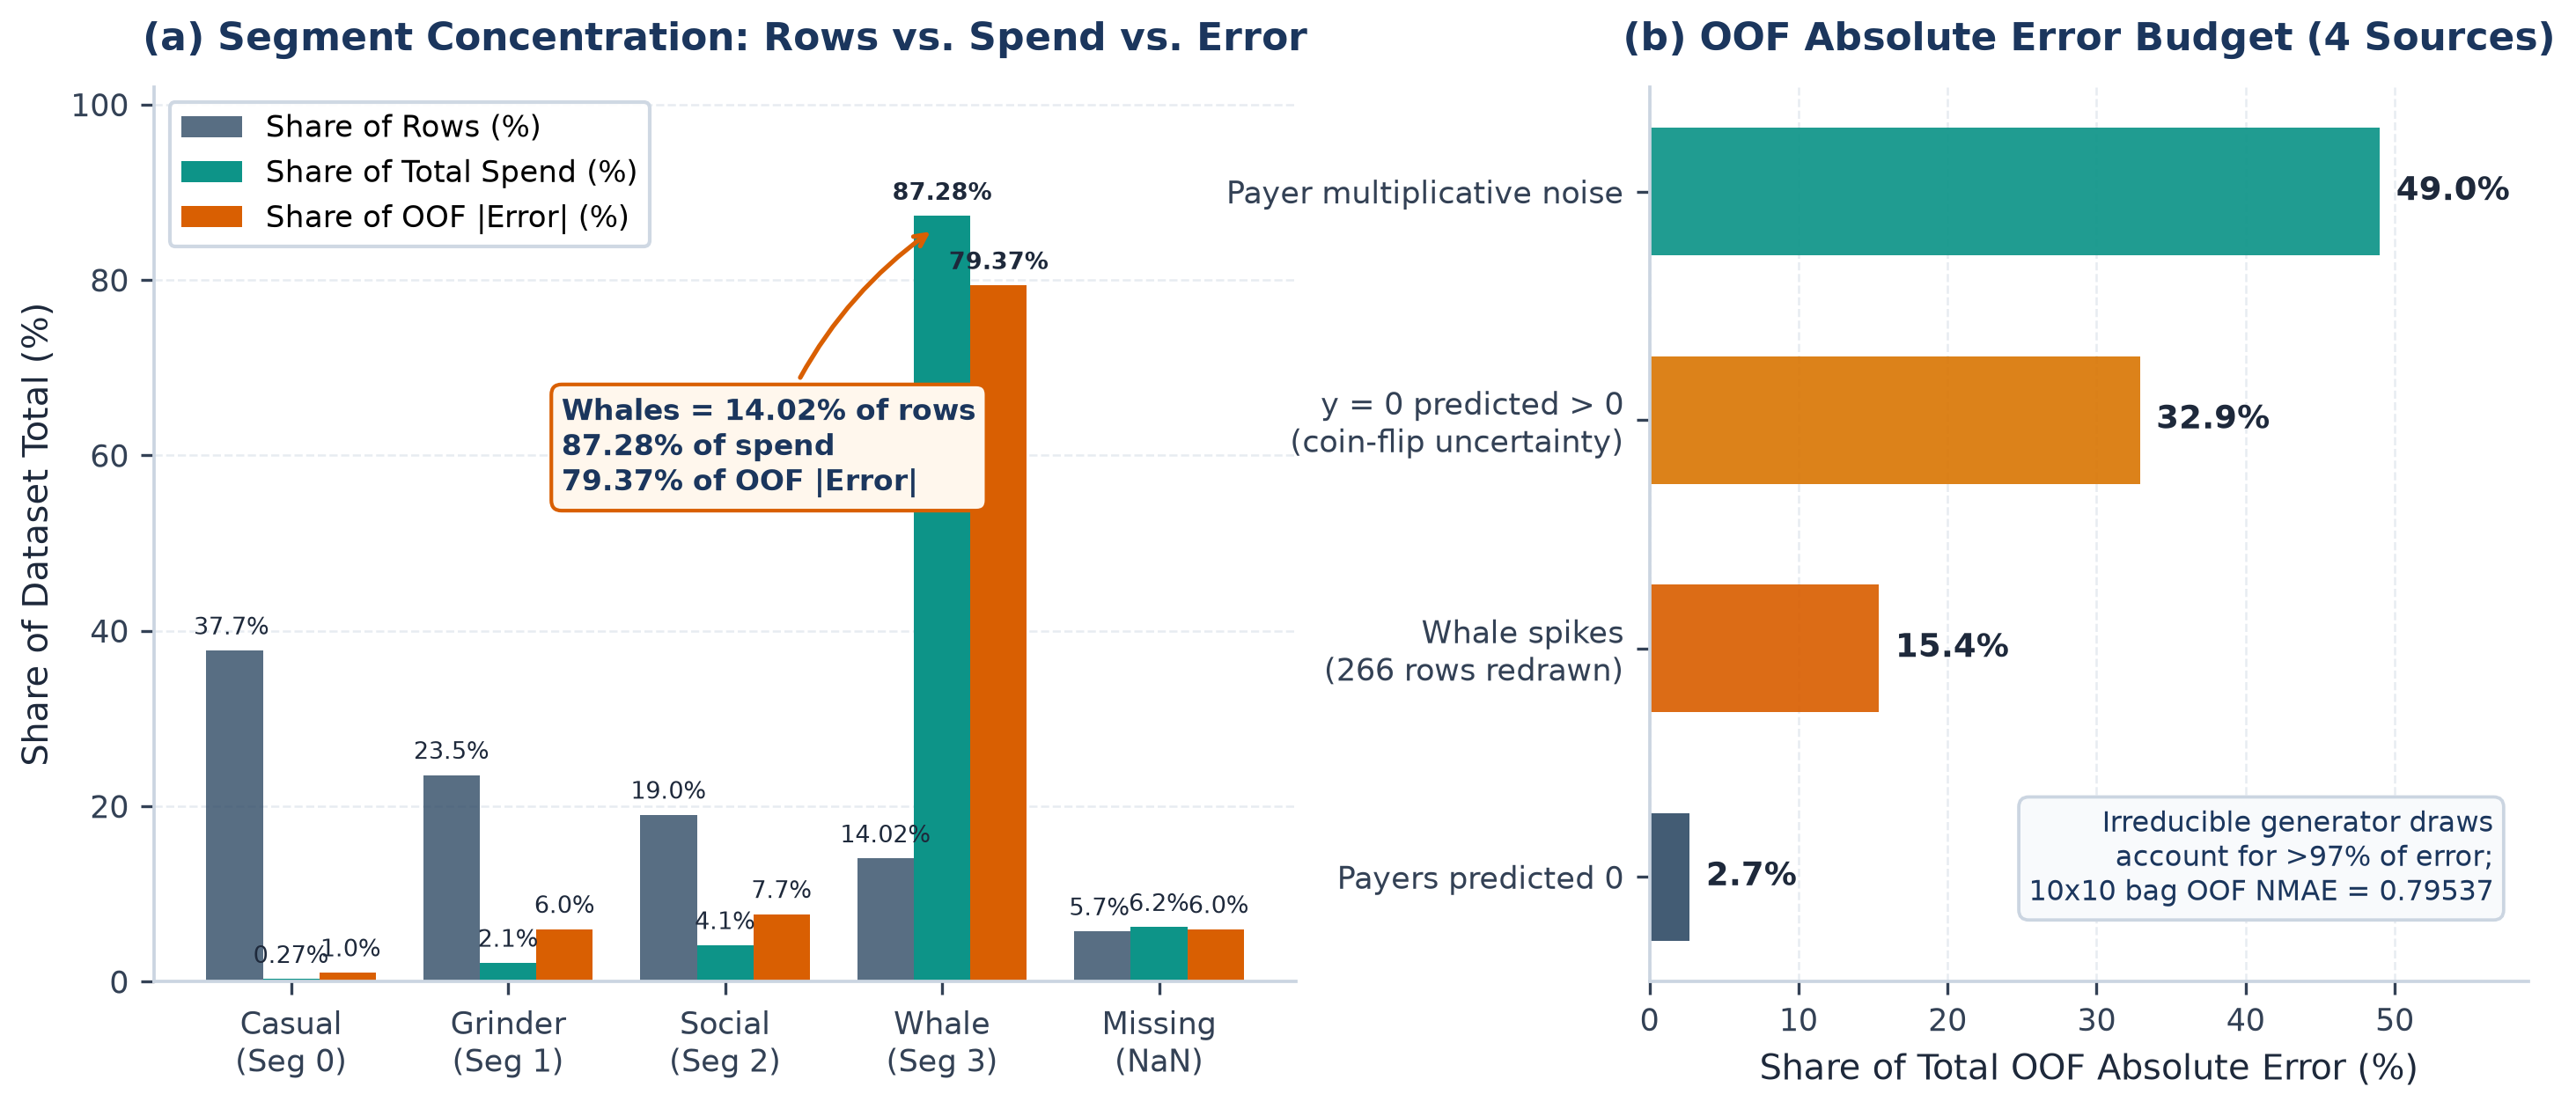
\includegraphics[width=0.98\textwidth]{figures/t3/fig_t3_whale_and_error_budget.png}
    \caption{(a) การกระจุกตัวของยอดใช้จ่ายและ OOF Absolute Error ในกลุ่ม Whale (\protect\feat{segment} = 3) ซึ่งมีเพียง 14.02\% ของแถวทั้งหมดแต่ครอง 87.28\% ของยอดใช้จ่ายและ 79.37\% ของความคลาดเคลื่อนรวม และ (b) งบประมาณความคลาดเคลื่อน OOF จำแนกตามแหล่งกำเนิด 4 ส่วน ซึ่งกว่า 97\% มาจากการสุ่มที่ลดทอนไม่ได้ของตัวกำเนิดข้อมูล}
    \label{fig:t3_whale_budget}
\end{figure}

\paragraph{2. เอกลักษณ์เชิงพีชคณิตและโครงสร้างตัวคูณใน Log-Space (Multiplicative DGP)}
\textbf{Claim:} ฟีเจอร์ทางการเงินภายในชุดข้อมูลมีความสัมพันธ์เชิงพีชคณิตแบบแม่นยำ และตัวแปรเป้าหมาย $y > 0$ ถูกสร้างจากฐาน \feat{prev\_month\_spending} คูณด้วยตัวคูณเชิงระดับขั้น (Step Factors) และสัญญาณรบกวนแบบสี่เหลี่ยมคางหมูที่มีขอบเขตจำกัด (Bounded Trapezoid Noise) \\
\textbf{Evidence:}
\begin{enumerate}
    \item \textbf{เอกลักษณ์เชิงพีชคณิตของฟีเจอร์:} ในทุกแถวที่ไม่เป็นค่าว่าง พบสมการเอกลักษณ์ 2 คู่ ได้แก่
    \begin{align*}
    \text{\texttt{historical\_spending}} &= \text{\texttt{total\_transactions}} \times \text{\texttt{avg\_transaction\_value}}, \\
    \text{\texttt{purchases\_on\_discount}} &= \text{\texttt{total\_transactions}} \times \text{\texttt{discount\_rate\_used}}
    \end{align*}
    นอกจากนี้ \feat{historical\_spending} ยังมีความสัมพันธ์เป็น \feat{prev\_month\_spending} $\times\, U(2.49, 3.35)$ ในทุกกลุ่ม ทำให้เมื่อทราบค่า \feat{prev\_month\_spending} แล้ว \feat{historical\_spending} แทบไม่เพิ่มข้อมูลส่วนต่างใหม่ในสัดส่วนฐาน (\feat{round9\_sonnet}: $\ln(\text{hist}/\text{prev}) \in [-1.21, -0.91]$) และพบว่า \feat{purchase\_frequency} กับ \feat{days\_since\_last\_purchase} เป็นการอ่านค่าจากระดับพฤติกรรมการซื้อแฝง (Latent Purchase Tier) เดียวกัน โดยมีสหสัมพันธ์ใน Log-space เท่ากับ $-0.64$
    \item \textbf{สมการกำเนิดตัวแปรเป้าหมาย:} สำหรับโอกาสการจ่ายเงิน $p(\mathbf{x})$ จะแปรผันเป็นฟังก์ชันขั้นบันไดตาม \feat{segment} (0.27 / 0.50 / 0.67 / 0.91 เมื่อไม่มีสิทธิ์ Premium), \feat{is\_premium\_member}, \feat{vip\_status} $\ge 3$, \feat{days\_since\_last\_purchase} $\le 15$ และ \feat{purchase\_frequency} $> 15$ โดยฤดูกาลรายเดือนไม่มีผลต่อ $p(\mathbf{x})$ ส่วนเมื่อ $y > 0$ กระบวนการสร้างข้อมูลเป็นไปตามสมการตัวคูณ:
    \begin{equation}
    \label{eq:t3_dgp}
    y = \text{\texttt{prev\_month\_spending}} \times \text{base}(\text{segment}) \times \prod_k \text{step\_factor}_k(\mathbf{x}) \times \varepsilon_{\text{trap}}
    \end{equation}
    โดยอัตราส่วนฐาน $\text{base}(\text{segment})$ (กรณีไม่มี Premium, VIP 0 และเดือนปกติ) คือ \textbf{1.10x} (Seg 0), \textbf{1.63x} (Seg 1), \textbf{1.82x} (Seg 2) และ \textbf{3.04x} (Seg 3) คูณด้วยตัวคูณร่วมทุกกลุ่ม ได้แก่ \feat{is\_premium\_member} ($\times 1.52$), \feat{vip\_status} ระดับ 1--5 ($\times 1.12 / 1.23 / 1.60 / 1.75 / 1.90$), จำนวน \feat{games\_played} เพิ่มขึ้นเกมละ $\times 1.07$, ปัจจัยฤดูกาลเดือน 0 และ 11 ($\times 1.26$) หรือเดือน 5 และ 6 ($\times 1.16$), \feat{days\_since\_last\_purchase} $< 15$ ($\times 1.16$) หรือ $> 45$ ($\times 0.80$), และ \feat{purchase\_frequency} ($\approx -20\%$ เมื่อต่ำกว่า 5 และ $+16\%$ เมื่อเกิน 17)
    \item \textbf{ความชันหนึ่งหน่วยใน Log-Space และพื้นความผันผวนแบบ Trapezoid:} เมื่อตรวจสอบความสัมพันธ์ $\ln(\text{\texttt{spending\_30d}})$ เทียบกับ $\ln(\text{\texttt{prev\_month\_spending}})$ บนผู้จ่ายเงินที่ทราบกลุ่มดังรูปที่~\ref{fig:t3_offset_linearity}(a) พบค่าสหสัมพันธ์เพียร์สันและความชันถดถอย (OLS Slope) ที่ใกล้เคียง $1.0$ อย่างยิ่งในทุกกลุ่ม ได้แก่ \textbf{Seg 0}: $r = 0.9611$, slope = $0.993$ (base $1.10\times$, median $1.20\times$); \textbf{Seg 1}: $r = 0.9335$, slope = $0.983$ (base $1.63\times$, median $1.93\times$); \textbf{Seg 2}: $r = 0.9355$, slope = $0.990$ (base $1.82\times$, median $2.32\times$); และ \textbf{Seg 3}: $r = 0.8823$, slope = $0.966$ (base $3.04\times$, median $4.74\times$) สำหรับส่วนความคลาดเคลื่อน OOF บน Seg 0--2 ในรูปที่~\ref{fig:t3_offset_linearity}(b) ค่า $\ln(y / Q_{50,\text{OOF}})$ มีส่วนเบี่ยงเบนมาตรฐานเพียง \textbf{$\text{sd} = 0.1504$} (ลดลงจาก $0.2982$ ของ $\ln(y/\text{prev})$ ดิบหลังลบมัธยฐานกลุ่ม) โดยข้อมูลถึง \textbf{99.27\%} อยู่ภายในขอบเขต $[0.66\times, 1.38\times]$ (หรือ $[-0.42, +0.32]$ ใน Log-space) ซึ่งเป็นรูปทรงความหนาแน่นแบบสี่เหลี่ยมคางหมูที่มีส่วนยอดราบในช่วง $[0.86\times, 1.10\times]$ อันเกิดจากผลคูณของตัวแปรสุ่ม Uniform สองตัว
    \item \textbf{Whale Spikes 266 แถว:} พบผู้จ่ายกลุ่ม Whale จำนวน \textbf{266 แถว} (1.7\% ของผู้จ่ายกลุ่ม Whale หรือ \textbf{0.26\%} ของชุดฝึกสอนทั้งหมด) ที่ถูกสุ่มค่า $y$ ใหม่ในช่วง \textbf{90,000--290,000 THB} (ตัดยอดไม่เกิน 300,000 THB) โดยไม่ขึ้นกับ \feat{prev\_month\_spending} และไม่สามารถทำนายได้จากฟีเจอร์ใดๆ (AUC การแยก Spike จากฟีเจอร์อยู่ที่ 0.58 ซึ่งเกิดจากกติกาคัดกรองเอง) นอกจากนี้ ยังยืนยันว่าไม่มีข้อมูลรั่วไหลจาก \feat{player\_id} หรือลำดับแถว (Spearman เทียบ $y$ เท่ากับ 0.004 และ zero-prediction AUC 0.497--0.499) ส่วนค่าว่างใน \feat{segment} (5.71\% ใน train และ 5.94\% ใน test) มีลักษณะ Missing Completely at Random (MCAR)
\end{enumerate}
\textbf{Implication:} การค้นพบสมการตัวคูณที่~\eqref{eq:t3_dgp} เปลี่ยนรูปปัญหาจากการให้ต้นไม้ตัดสินใจจำลองระนาบเส้นทแยงมุม $y \propto \text{\texttt{prev\_month\_spending}}$ ไปเป็นการเรียนรู้เฉพาะตัวคูณ $\ln(y / \text{prev})$ โดยล็อกความชันไว้ที่ $1.0$

\begin{figure}[htbp]
    \centering
    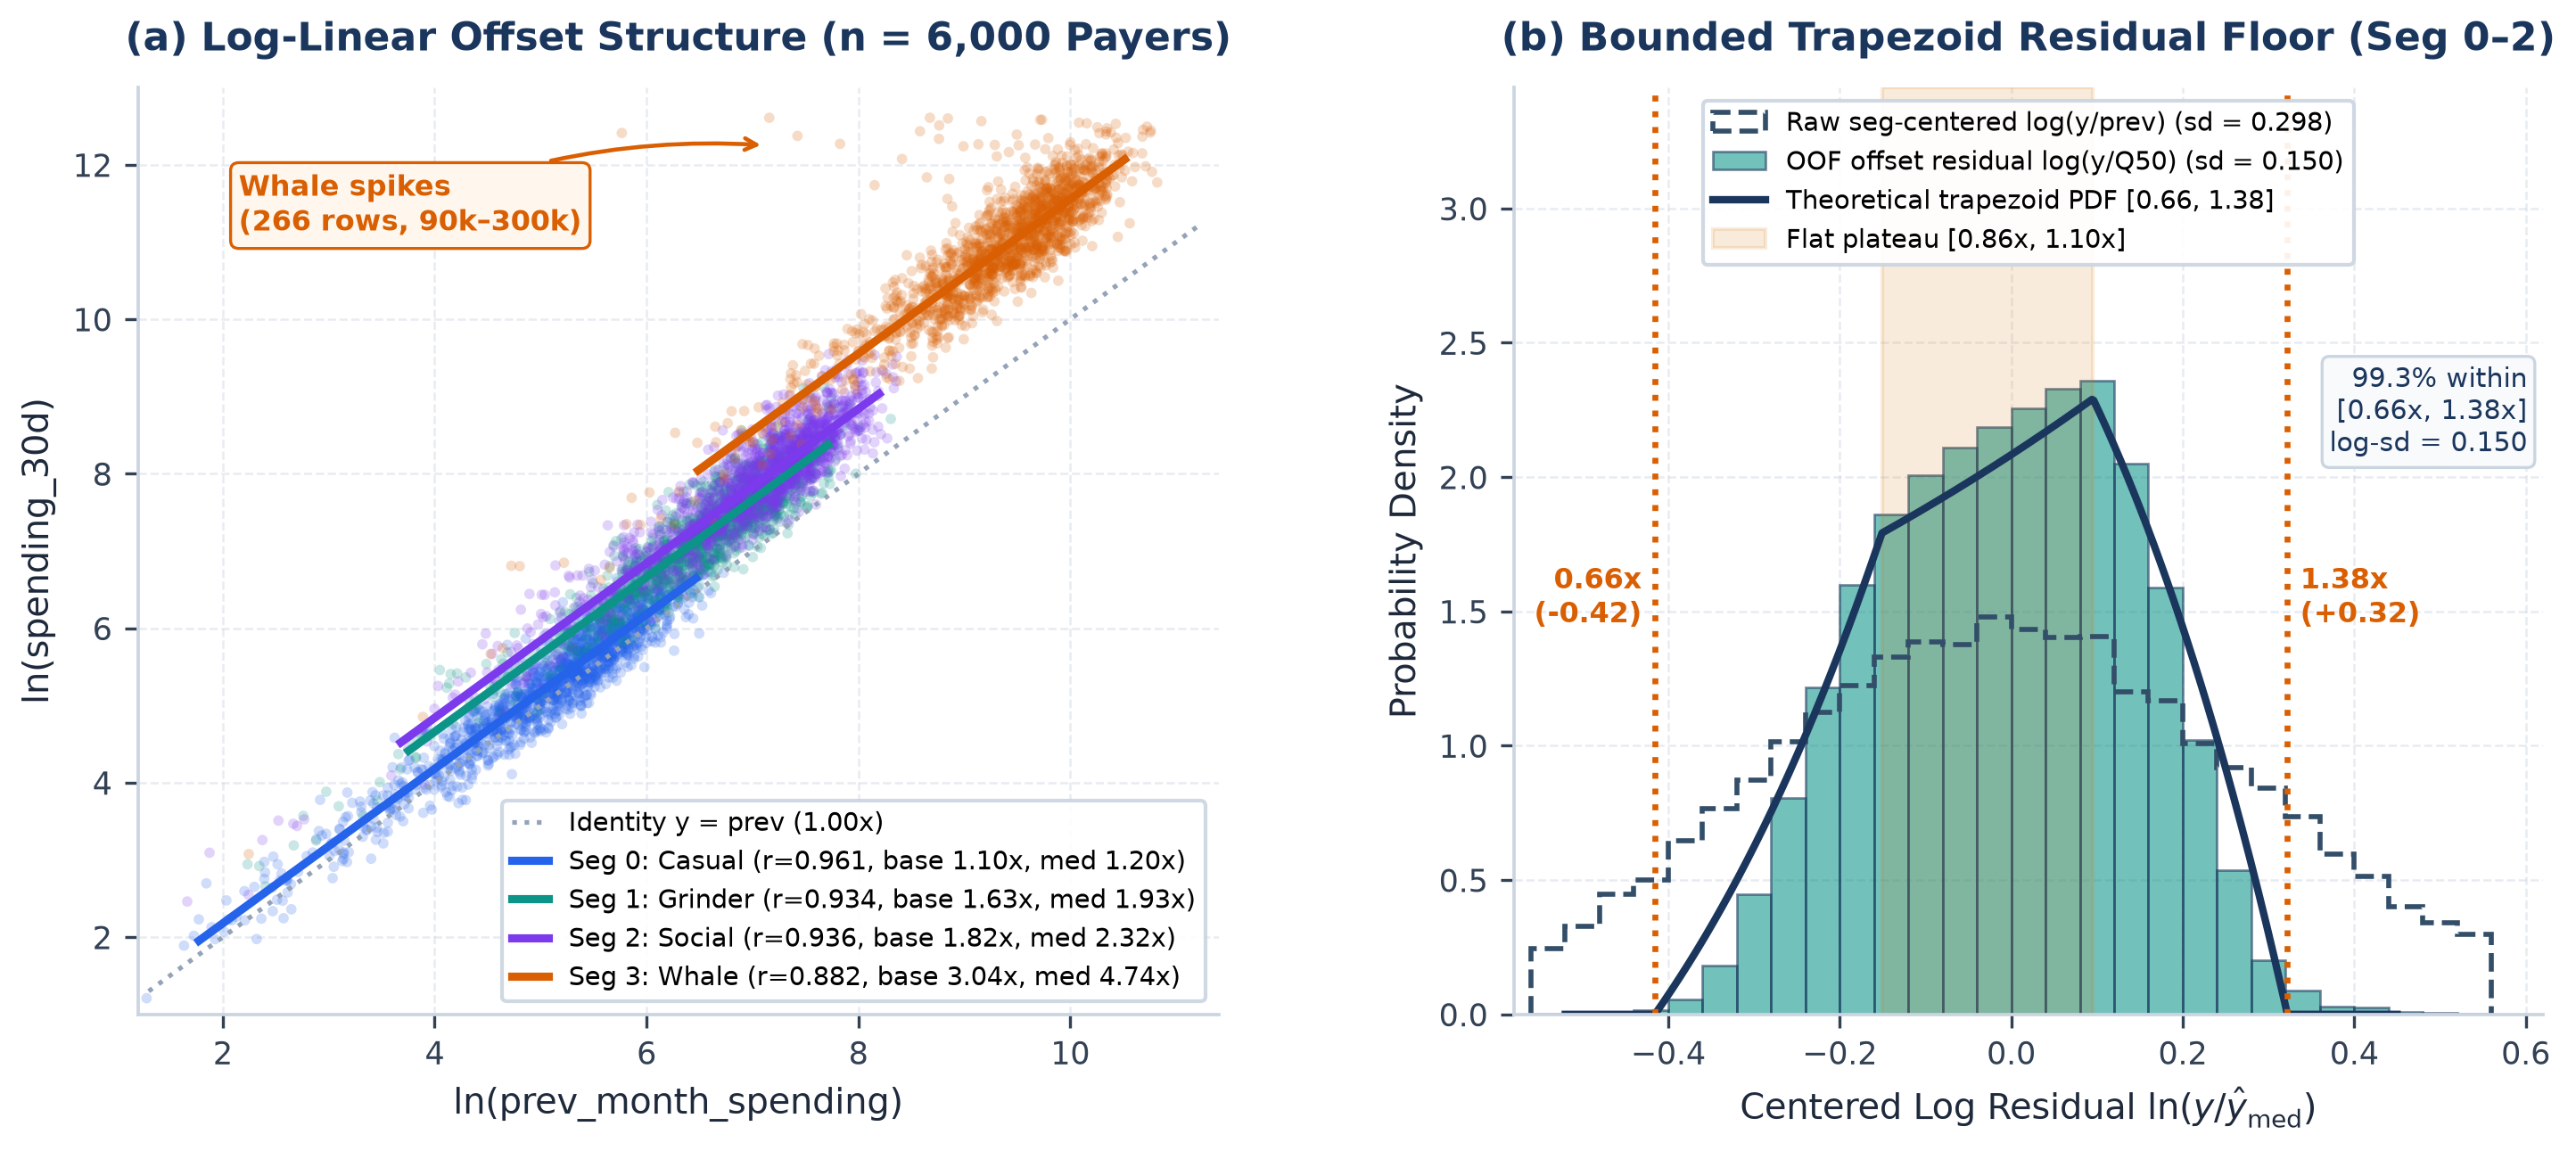
\includegraphics[width=0.98\textwidth]{figures/t3/fig_t3_offset_linearity.png}
    \caption{(a) ความสัมพันธ์เชิงเส้นความชันใกล้ 1.0 ระหว่าง $\ln(\text{\texttt{spending\_30d}})$ กับ $\ln(\text{\texttt{prev\_month\_spending}})$ ในผู้จ่ายเงิน 6,000 ราย (สุ่มกลุ่มละ 1,500 ราย) พร้อมกลุ่ม Whale Spikes 266 แถวด้านบนซ้าย และ (b) การแจกแจงของ Log-Residual ใน Seg 0--2 ซึ่งโมเดล OOF Offset ลด $\text{sd}$ จาก $0.298$ ลงเหลือ $0.150$ และเกาะตามทฤษฎี Bounded Trapezoid PDF ในช่วง $[0.66\times, 1.38\times]$ ถึง $99.27\%$}
    \label{fig:t3_offset_linearity}
\end{figure}

\begin{insightbox}[เหตุใดการเปลี่ยน Target เป็น Log-Ratio Offset จึงปลดล็อกประสิทธิภาพของ Tree Models]
ดังที่เห็นในรูปที่~\ref{fig:t3_offset_linearity}(a) ค่า \feat{spending\_30d} มีช่วงพิสัยกว้างหลายอันดับขนาดและแปรผันตรงตาม \feat{prev\_month\_spending} ด้วยความชันใน Log-space เกือบเท่ากับ 1.0 ในทุกกลุ่ม ($0.966$--$0.993$) หากฝึกต้นไม้ตัดสินใจเพื่อทำนาย $\ln(y)$ โดยตรง ต้นไม้ซึ่งแบ่งขอบเขตด้วยเส้นตั้งฉาก (Axis-Aligned Splits) ต้องสิ้นเปลืองความลึกและจำนวนใบมหาศาลเพียงเพื่อสร้างขั้นบันไดเลียนแบบเส้นทแยงมุม $y = \text{prev}$ เมื่อเราย้าย $\ln(\text{\texttt{prev\_month\_spending}})$ ไปเป็น Offset คงที่ แล้วให้โมเดลทำนายเฉพาะ Residual $r = \ln(y) - \ln(\text{\texttt{prev\_month\_spending}})$ ความแปรปรวนที่ต้นไม้ต้องอธิบายจะถูกบีบลงเหลือเฉพาะ Step Factors ไม่กี่ตัวจนเข้าชนพื้นสัญญาณรบกวนแบบ Trapezoid ($\text{sd} = 0.1504$) ดังรูปที่~\ref{fig:t3_offset_linearity}(b) ได้โดยตรง
\end{insightbox}

% ----------------------------------------------------------------------
\subsubsection{การเตรียมข้อมูลและ Feature Engineering}
\label{subsubsec:t3_fe}

กระบวนการเตรียมข้อมูลทั้งหมดถูกออกแบบภายใต้กติกา \textbf{Test-Free Inference} อย่างเคร่งครัดใน \feat{t3/research/common.py} โดยไม่นำแถวของ \feat{test.csv} หรือตัวแปรเป้าหมายมาใช้ในการประมาณค่าใดๆ มีขั้นตอนดังนี้:

\begin{enumerate}
    \item \textbf{การเติมค่าว่างด้วยสมการเอกลักษณ์ (\feat{exact\_fill}):} วนซ้ำ 3 รอบโดยใช้กฎผกผันทั้ง 6 ข้อจากสมการเอกลักษณ์ 2 คู่ระหว่าง \feat{historical\_spending}, \feat{total\_transactions}, \feat{avg\_transaction\_value}, \feat{purchases\_on\_discount} และ \feat{discount\_rate\_used} (ป้องกันการหารด้วยศูนย์) ช่วยลดอัตราค่าว่างในกลุ่มฟีเจอร์เอกลักษณ์ 5 คอลัมน์จากเดิมเฉลี่ย \textbf{5.8\%} (5.76\%--5.87\% หรือ 30,279 ช่องในชุดฝึกสอน) ลงเหลือเพียง \textbf{0.4\%} (0.10\%--0.44\% หรือเฉลี่ย 0.34\% เหลือเพียง 1,752 ช่องในชุดฝึกสอน และ 0.08\%--0.45\% ในชุดทดสอบ)
    \item \textbf{ตัวเติมค่าว่าง \feat{segment} แบบ Train-Only:} สำหรับแถวที่ขาดค่า \feat{segment} (5,935 แถว หรือ 5.71\% ในชุดฝึกสอน และ 5.94\% ในชุดทดสอบ) เราฝึก \feat{XGBClassifier} (\feat{multi:softprob}, \feat{max\_depth=6}, \feat{learning\_rate=0.02}, early stopping 100 บนชุดแบ่ง 10\%) โดยใช้ \textbf{เฉพาะแถวในชุดฝึกสอนที่ทราบ \feat{segment} (98,065 แถว) และห้ามใช้เป้าหมาย \feat{spending\_30d}} ได้ความแม่นยำบน Holdout ถึง \textbf{0.929} (ค่าจริง 0.9286 ซึ่งใกล้เพดาน Bayes ของฟีเจอร์แล้ว) พร้อมสร้างฟีเจอร์ \feat{seg\_imputed} (ตัวบ่งชี้การเติมค่า) และ \feat{p\_whale} (ความน่าจะเป็นที่จะอยู่ใน Seg 3: เท่ากับ 1.0/0.0 เมื่อทราบกลุ่ม และใช้ค่าความน่าจะเป็น $P(\text{seg}=3)$ จากตัวเติมเมื่อค่าหายไป)
    \item \textbf{ฟีเจอร์เชิงวิศวกรรมแบบ Deterministic (รวม 49 ฟีเจอร์):} จากฟีเจอร์ดิบ 32 ตัวแปร เพิ่มฟีเจอร์อัตราส่วนและลอการิทึมจากสายงาน \feat{v4} จำนวน 11 ตัวแปร ได้แก่ \feat{hist\_per\_day}, \feat{tx\_per\_day}, \feat{exp\_monthly\_spend}, \feat{prev\_vs\_hist}, \feat{prev\_x\_freq}, \feat{recency\_ratio}, \feat{play\_per\_session}, \feat{log\_historical\_spending}, \feat{log\_prev\_month\_spending}, \feat{log\_avg\_transaction\_value} และ \feat{n\_missing} ร่วมกับ \feat{seg\_imputed} และ \feat{p\_whale} เป็น 45 ฟีเจอร์ จากนั้นเพิ่มฟีเจอร์ Log-Ratio ของฟังก์ชัน \feat{extra\_feats} อีก 4 ตัวแปร ได้แก่ \feat{lprev\_minus\_lhist}, \feat{l\_atv\_x\_freq}, \feat{l\_hist\_per\_tx} และ \feat{l\_hist\_per\_age} รวมเป็น 49 ฟีเจอร์เต็มรูปแบบ (ทั้งนี้ จากการทดสอบ \feat{R8-05} พบว่ามีถึง 36 จาก 49 ฟีเจอร์ที่ CatBoost ให้ความสำคัญต่ำกว่า 0.5\% และการตัดเหลือ 13 ฟีเจอร์หลักให้คะแนนเท่าเดิมที่ $+0.00008 \pm 0.00039$ แสดงให้เห็นว่าโมเดลต้นไม้สามารถเพิกเฉยต่อฟีเจอร์รบกวนได้เอง)
\end{enumerate}

\paragraph{กรณีศึกษาเชิงวินัย (Negative A/B Case Study): กฎ \feat{is\_premium\_member = (vip\_status >= 3)}}
จากการตรวจสอบความสอดคล้องของข้อมูลใน \feat{work/insight/c06\_t3\_premium\_fill.py} ถึง \feat{c08\_t3\_fill\_ab.py} ทีมงานค้นพบเอกลักษณ์ใหม่ที่มีความแม่นยำ 100\% คือ \feat{is\_premium\_member = (vip\_status >= 3)} โดยไม่มีข้อยกเว้นเลยแม้แต่แถวเดียว (\textbf{0 exceptions} จาก 97,000+ แถวที่ทราบค่าทั้งคู่) ซึ่งสามารถนำไปเติมค่า \feat{is\_premium\_member} ที่หายไปได้ถึง 5,715 แถว และกำหนดขอบเขต \feat{vip\_lo}/\feat{vip\_hi} ได้อีก 5,856 แถว
\begin{itemize}
    \item \textbf{ผลทดสอบ Proxy Metric (\feat{c06}):} เมื่อทดสอบด้วยโมเดล LightGBM แบบเร็ว (2$\times$5 folds) เฉพาะแถวที่ขาดค่า \feat{is\_premium\_member} พบว่าค่าเฉลี่ย $|\text{log residual}|$ ของผู้จ่ายเงินลดลงถึง \textbf{-4\%} (จาก 0.1460 เหลือ 0.1399) ค่าเฉลี่ยผู้จ่ายทั้งหมดดีขึ้นจาก 0.14075 เป็น 0.14028 และ pay log-loss ลดลงจาก 0.55316 เป็น 0.55293
    \item \textbf{ผลทดสอบ A/B บน Pipeline จริง (\feat{c08}):} แต่เมื่อนำการเติมค่าและฟีเจอร์ขอบเขตดังกล่าวไปทดสอบแบบ A/B บนโมเดลจริง (LightGBM $p$ + CatBoost \feat{d4} MultiQuantile บน Folds เดียวกัน) คะแนน OOF NMAE กลับได้ \textbf{0.79499} เทียบกับ \textbf{0.79506} เมื่อไม่เติม (\textbf{-0.00007}, ดีขึ้นเพียง 2 จาก 5 folds) เนื่องจาก CatBoost สามารถเรียนรู้เงื่อนไข Premium โดยตรงจาก \feat{vip\_status} และฟีเจอร์ร่วมอื่นๆ ได้อยู่แล้ว การเติมค่าจึงไม่ช่วยเพิ่มสัญญาณในโมเดลปลายทางและถูก\textbf{ปฏิเสธ (Rejected)} เพื่อยึดวินัยการตัดสินใจจาก CV ของ Pipeline จริงเท่านั้น
\end{itemize}

% ----------------------------------------------------------------------
\subsubsection{การออกแบบโมเดล Hurdle + Offset CatBoost MultiQuantile และเหตุผลเชิงวิศวกรรม}
\label{subsubsec:t3_model_design}

จากสมการความเหมาะสมของ MAE ที่~\eqref{eq:t3_hurdle_quantile} และสมการ DGP ที่~\eqref{eq:t3_dgp} สถาปัตยกรรมสุดท้ายของ Task 3 ถูกออกแบบเป็นระบบ \textbf{Two-Stage Hurdle Model} ที่มี 2 ขั้นตอนหลักและไม่มีการจูนน้ำหนัก Post-Hoc ใดๆ:

\begin{enumerate}
    \item \textbf{ขั้นตอนที่ 1 — ตัวจำแนกโอกาสการจ่ายเงิน $p = P(y > 0 \mid \mathbf{x})$:} ใช้ \feat{LGBMClassifier} (\feat{learning\_rate=0.03}, \feat{num\_leaves=63}, \feat{min\_child\_samples=40}, \feat{subsample=0.8}, \feat{colsample\_bytree=0.7}, \feat{reg\_lambda=2.0}, early stopping 100 รอบบนชุดแบ่งย่อย 10\% ภายใน training fold) เฉลี่ยความน่าจะเป็นจาก 10 seeds (\feat{lgbh\_log} และ \feat{clf\_s1}--\feat{clf\_s9}) ได้ค่า OOF ROC-AUC รวม \textbf{0.7844} (seed เดียว 0.7838, 3-seed 0.7841) อย่างไรก็ตาม จากการวิเคราะห์เชิงลึกพบว่าพลังการจำแนกเกือบทั้งหมดมาจากการแยกอัตราการจ่าย \textit{ระหว่าง} กลุ่มผู้เล่น (7.15\%--72.44\% zero rate) ขณะที่การจำแนกว่าผู้เล่นคนหนึ่งจะจ่ายหรือไม่จ่าย \textit{ภายใน} กลุ่มเดียวกันมีค่า AUC เพียง \textbf{0.55--0.63} (Seg 0: 0.6051, Seg 1: 0.6283, Seg 2: 0.6011, Seg 3: 0.5665) ซึ่งใกล้เคียงการสุ่ม จึงอธิบายได้ว่าเหตุใดการเปลี่ยนตัวจำแนกไปใช้ CatBoost \feat{d6}/\feat{d4} (AUC 0.78446 / 0.78443) หรือ XGBoost \feat{d5} (0.78413) จึงเพิ่ม OOF NMAE เพียง +0.00002 เท่านั้น
    \item \textbf{ขั้นตอนที่ 2 — CatBoost MultiQuantile บน Unit-Slope Offset Residual:} ฝึกเฉพาะแถวผู้จ่ายเงิน ($y > 0$) ในแต่ละ training fold เพื่อทำนาย 11 ระดับควอนไทล์พร้อมกันผ่านฟังก์ชันสูญเสีย \feat{MultiQuantile:alpha=0.02,0.05,0.1,0.15,0.2,0.25,0.3,0.35,0.4,0.45,0.5} โดยเป้าหมายที่ใช้ฝึกคือ Residual เทียบกับ Offset ที่ล็อกสัมประสิทธิ์ไว้เท่ากับ 1 (\textit{Unit-Slope Offset}):
    \begin{equation}
    \label{eq:t3_offset_target}
    r_i = \ln(y_i) - \text{offset}(\mathbf{x}_i), \qquad
    \text{offset}(\mathbf{x}_i) =
    \begin{cases}
    \ln(\text{\texttt{prev\_month\_spending}}_i), & \text{หากไม่เป็นค่าว่าง} \\
    \ln(\text{\texttt{historical\_spending}}_i) - 1.05, & \text{หาก }\text{\texttt{prev}}\text{ ว่าง} \\
    6.5, & \text{หากทั้งคู่ว่าง}
    \end{cases}
    \end{equation}
    ตัวแบบใช้ \feat{CatBoostRegressor} โครงสร้างต้นไม้สมมาตร (\feat{SymmetricTree}) ความลึก \textbf{\feat{depth=4}}, \feat{learning\_rate=0.05}, \feat{l2\_leaf\_reg=3}, \feat{od\_type='Iter'}, \feat{od\_wait=200} บนชุดแบ่งย่อย 10\% ภายใน training fold จากนั้นแปลงควอนไทล์ที่ทำนายได้กลับเป็นสเกลบาทพร้อมเรียงลำดับป้องกัน Quantile Crossing:
    \[
    \hat{Q}_{\alpha}(y_i \mid y_i > 0) = \exp\!\Big(\text{sort}_{\alpha}\big(\hat{Q}_{\alpha}(r_i)\big) + \text{offset}(\mathbf{x}_i)\Big)
    \]
    \item \textbf{การรวมผลแบบ 10$\times$10 Seed Bagging (\feat{bag\_q10p10}) และ Hurdle Median:} เฉลี่ยความน่าจะเป็น $\bar{p}$ จาก LightGBM 10 seeds และหาค่า \textbf{Geometric Mean} ของควอนไทล์ $\bar{Q}_{\alpha} = \exp\!\left(\frac{1}{10}\sum_{s=0}^{9}\ln \hat{Q}_{\alpha}^{(s)}\right)$ จาก CatBoost \feat{d4} 10 seeds (\feat{cbq\_d4}, \feat{cbq\_d4s1}--\feat{cbq\_d4s9}) ก่อนนำเข้ากฎ Hurdle Mixture Median ที่~\eqref{eq:t3_hurdle_quantile}: หาก $\bar{p} \le 0.5$ ทำนาย $0.0$ มิฉะนั้นคำนวณ $q = \text{clip}(1 - \frac{1}{2\bar{p}}, 0.02, 0.50)$ แล้วประมาณค่าเชิงเส้น (Linear Interpolation) ระหว่าง 11 ระดับควอนไทล์ของ $\bar{Q}$ พร้อมจำกัดช่วงคำตอบไว้ที่ $[0, 300{,}000]$
\end{enumerate}

\begin{decisionbox}[เหตุผลเชิงวิศวกรรม: Unit-Slope Offset vs. Fitted Offsets และ Shallow Symmetric Trees]
\begin{enumerate}
    \item \textbf{เหตุใด Unit-Slope Offset จึงชนะ Fitted Linear/Ridge Offsets:} ในสมการ DGP ที่~\eqref{eq:t3_dgp} ความสัมพันธ์ระหว่าง $\ln y$ และ $\ln(\text{\texttt{prev}})$ มีความชันเท่ากับ $1.0$ พอดี หากใช้ Linear Regression (\feat{E08}: OOF \textbf{0.79223}) หรือ Ridge รายกลุ่ม (\feat{E10}: OOF \textbf{0.79283}) เป็น Offset แทนค่าสัมประสิทธิ์ $1.0$ (\feat{E07}: OOF \textbf{0.79405}) ความคลาดเคลื่อนจาก Whale Spikes 266 แถวและพฤติกรรม Mean-Regression ของกำลังสองน้อยสุดจะทำให้ความชันที่ประมาณได้เพี้ยนจากเส้น 1:1 และสร้าง Residual ที่ยังมีแนวโน้มเอียงหลงเหลือให้ต้นไม้ต้องซ่อมแซม ขณะที่ Unit-Slope Offset ไม่ใช้การประมาณค่าบนเป้าหมาย ลดโอกาส Overfitting เป็นศูนย์ และเพิ่ม OOF ได้ถึง $+0.0023$ ใน XGBoost และ $+0.0039$ ใน LightGBM
    \item \textbf{เหตุใดต้นไม้ตื้นแบบ Symmetric Tree (\feat{CatBoost d4}) จึงเหนือกว่าต้นไม้ลึกและ XGB/LGB:} Residual $r_i$ เกิดจากผลบวกใน Log-space ของ Step Factors ไม่กี่ตัวที่ทำงานสอดคล้องกันในทุก Segment แทบไม่มีปฏิสัมพันธ์ซับซ้อนระดับลึก การเพิ่มความลึกของต้นไม้จึงรังแต่จะจำสัญญาณรบกวนแบบ Trapezoid (\feat{CatBoost} \feat{d4}: \textbf{0.79505} $\approx$ \feat{d3}: \textbf{0.79507} $\approx$ \feat{d6}: \textbf{0.79497} $>$ \feat{d8}: \textbf{0.79434}/\textbf{0.79449}; ขณะที่ \feat{XGB} \feat{d5}: \textbf{0.79424} $\ge$ \feat{d7}: \textbf{0.79405} $>$ \feat{d9}: \textbf{0.79321}) อีกทั้งโครงสร้าง \feat{SymmetricTree} ของ CatBoost ที่ใช้เงื่อนไขแบ่งเดียวกันตลอดทั้งชั้นความลึก (16 Leaves ที่ \feat{d4}) ทำหน้าที่เป็นตัวกรองโครงสร้างแบบ Global Step-Factor โดยธรรมชาติ ซึ่งได้รับการยืนยันจากการค้นหา Optuna 31 รอบ (\feat{R6-01}) ที่พบว่าการตั้งค่าที่ชนะทั้งหมดเป็น \feat{SymmetricTree} ความลึก 3--4 ทั้งสิ้น ส่วน \feat{Depthwise} และความลึก $\ge 5$ ให้ผลด้อยกว่าทั้งหมด
\end{enumerate}
\end{decisionbox}

% ----------------------------------------------------------------------
\subsubsection{กลยุทธ์การวัดผล ลำดับการทดลอง และผลลัพธ์สุดท้าย}
\label{subsubsec:t3_progression}

การวัดผลทั้งหมดใช้ \textbf{5-Fold StratifiedKFold (seed 42)} ตาม \feat{common.folds\_v4} โดยแบ่งชั้นจากกลุ่มผู้ไม่จ่ายเงิน ($y=0$) และ 4 ควอไทล์ของผู้จ่ายเงิน ($y>0$) และเพื่อป้องกันอคติจากการแบ่งชุดข้อมูล ทีมงานได้ทดสอบทำซ้ำบนชุดแบ่ง Fold ใหม่ทั้งหมด (\feat{FOLD\_SEED=7}, \feat{R2-09}) พบว่าสูตรสุดท้ายทำคะแนนได้ 0.79531 เทียบกับโมเดล XGB แบบไม่มี Offset ที่ 0.79183 คิดเป็น Paired Gain \textbf{$+0.00348 \pm 0.00045$} (เป็นบวกครบทั้ง 5/5 Folds) สอดคล้องกับ $+0.00344$ บน Fold เดิม ยืนยันว่าผลกำไรไม่ได้เกิดจากความบังเอิญของการแบ่ง Fold

ตารางที่~\ref{tab:t3_progression} และรูปที่~\ref{fig:t3_progression_ceiling} แสดงลำดับความก้าวหน้าของระบบตั้งแต่ Baseline จนถึงโมเดลสุดท้าย:
\begin{itemize}
    \item เริ่มจากจุดอ้างอิงพื้นฐาน All-Zero (0.50000), HistGradientBoosting (HGB) แบบ Direct MAE (0.7809) และ HGB Two-Stage (0.7843)
    \item สายงาน \feat{v4} ที่ใช้ XGBoost MultiQuantile บน $\ln(1+y)$ (\feat{D\_q}) ทำคะแนน OOF ได้ 0.79169 และเมื่อรวมโมเดลภายในสายงาน \feat{v4} ด้วย Nested LAD Blending อย่างซื่อสัตย์ (\feat{E02}) ได้เป็น \textbf{Honest Baseline = 0.79191} (หมายเหตุ: ค่า 0.79195 หรือ 0.7925 จาก \feat{v4}+NN เดิมเกิดจากการจูนน้ำหนักแบบ In-Sample บน OOF เดียวกัน จึงไม่นำมาใช้เป็นฐานอ้างอิง)
    \item การเปลี่ยนเป้าหมายของ XGBoost เป็น Unit-Slope Offset $\ln(y / \text{prev})$ (\feat{E06}) ยกระดับ OOF กระโดดขึ้นเป็น \textbf{0.79391} และเพิ่มเป็น 0.79405 เมื่อเสริม 4 \feat{extra\_feats} (\feat{E07})
    \item การเปลี่ยนจาก XGBoost เป็น CatBoost MultiQuantile ตื้นความลึก 4 (\feat{E30}, single seed) ยกระดับขึ้นอีกเป็น \textbf{0.79505} (ลด Error Ratio ในกลุ่ม Whale จาก 0.2385 ใน \feat{v4} ลงเหลือ 0.2330 ในสูตรสุดท้าย)
    \item การทำ Seed Bagging แบบ 3$\times$3 (\feat{bag\_q3p3}, \feat{E35}) ได้ OOF \textbf{0.79529} (Fold Mean $0.79534 \pm 0.00759$) ซึ่งชนะ Honest Baseline \feat{v4} อย่างมีนัยสำคัญทุก Fold ด้วย Paired Gain \textbf{$+0.00337 \pm 0.00043$} (ราย Fold: $+0.0038, +0.0033, +0.0038, +0.0026, +0.0034$)
    \item การขยายเป็น \textbf{10$\times$10 Seed Bagging (\feat{bag\_q10p10})} บน Kaggle CPU (\feat{t3/kaggle/task3-seedbag10/task3\_seedbag10.py}, เวลาประมวลผลรวม 0.93 ชั่วโมง) ทำสถิติ OOF สูงสุดที่ \textbf{0.79537} (Fold Mean \textbf{$0.79542 \pm 0.00760$}, อัตราการทำนายศูนย์ 50.32\%) โดยไม่ใช้การจูนน้ำหนักหรือ Threshold ใดๆ เลย (นอกจากนี้ ยังมีทางเลือก \feat{robust\_oof} ซึ่งเฉลี่ย Geometric Mean แบบถ่วงเท่ากัน 4 ตระกูลคือ CatBoost \feat{d4}/\feat{d3}/\feat{d6} และ XGBoost \feat{d5} ได้ OOF \textbf{0.79526} และมีสหสัมพันธ์บน Test กับไฟล์หลักถึง \textbf{0.99997})
\end{itemize}

\begin{table}[htbp]
\centering
\caption{วิวัฒนาการของโมเดล Task 3 บน 5-Fold StratifiedKFold (\protect\feat{folds\_v4}) และชุดทดสอบ}
\label{tab:t3_progression}
\footnotesize
\setlength{\tabcolsep}{4pt}
\begin{tabularx}{\textwidth}{@{}p{4.8cm}cccX@{}}
\toprule
\textbf{โมเดล / จุดเปลี่ยนสำคัญ} & \textbf{OOF NMAE} & \textbf{Fold Mean $\pm$ SD} & \textbf{เทียบ Honest v4} & \textbf{คำอธิบายเชิงวิศวกรรม} \\
\midrule
All-Zero Baseline & 0.50000 & -- & $-0.29191$ & ทำนาย $\hat{y}_i = 0$ ทุกแถว ($E/Y = 1$) \\
HGB Direct MAE (\feat{t3\_hgb\_cv.json}) & 0.7809 & -- & $-0.0110$ & โมเดลจุดเดียว ไม่แยกกลไกศูนย์ \\
HGB Two-Stage Baseline & 0.7843 & -- & $-0.0076$ & แยกตัวจำแนกศูนย์กับปริมาณ \\
\feat{v4} XGB MultiQuantile \feat{D\_q} (\feat{E00}) & 0.79169 & $0.79174 \pm 0.0075$ & $-0.00022$ & ทำนาย 12 ควอนไทล์บน $\ln(1+y)$ \\
\textbf{\feat{v4} Honest Nested LAD (\feat{E02})} & \textbf{0.79191} & $0.79196 \pm 0.0077$ & \textbf{ฐานอ้างอิง} & ผสาน 5 โมเดล \feat{v4} แบบ Nested LP \\
XGB \feat{d7} + Offset $\ln(y/\text{prev})$ (\feat{E06}) & 0.79391 & $0.79396 \pm 0.0076$ & $+0.00200$ & ตัดภาระต้นไม้ในการจำลองเส้น 1:1 \\
XGB \feat{d7} + Offset + 4 \feat{extra\_feats} (\feat{E07}) & 0.79405 & $0.79410 \pm 0.0077$ & $+0.00214$ & เสริม Log-Ratio ฟีเจอร์ \\
CatBoost \feat{d4} Offset Single (\feat{E30}) & 0.79505 & $0.79510 \pm 0.00755$ & $+0.00314$ & ต้นไม้สมมาตรตื้นจับ Step Factors \\
\feat{robust\_oof} Equal 4-Family (\feat{R5-04}) & 0.79526 & $0.79531 \pm 0.0076$ & $+0.00335$ & CB \feat{d4/d3/d6} + XGB \feat{d5} อย่างละ 1/4 \\
CatBoost \feat{d4} 3$\times$3 Bag (\feat{bag\_q3p3}) & 0.79529 & $0.79534 \pm 0.00759$ & $+0.00337^*$ & ชนะครบ 5/5 Folds ($\pm 0.00043$) \\
CatBoost \feat{d4} 3$\times$10 Bag (\feat{bag\_q3p10}) & 0.79531 & $0.79535 \pm 0.00758$ & $+0.00340$ & เพิ่ม Seed ตัวจำแนกเป็น 10 \\
CatBoost \feat{d4} 10$\times$3 Bag (\feat{bag\_q10p3}) & 0.79535 & $0.79540 \pm 0.00761$ & $+0.00344$ & เพิ่ม Seed ควอนไทล์เป็น 10 \\
\textbf{Final 10$\times$10 Bag (\feat{bag\_q10p10})} & \textbf{0.79537} & $\mathbf{0.79542 \pm 0.00760}$ & \textbf{$+0.00346$} & \textbf{ส่งใช้งานจริง; $E/Y = 0.2573$} \\
\midrule
In-Sample Train Score (\feat{R6-04}) & 0.80356 & -- & $+0.01165$ & ฟิตและวัดบน Train เดียวกัน (เพดาน Noise) \\
\bottomrule
\end{tabularx}
\par\vspace{2pt}
{\footnotesize $^*$ ค่า Paired Gain ราย Fold ของ \feat{bag\_q3p3} เทียบ \feat{E02} คือ $+0.00337 \pm 0.00043$ (บวกทั้ง 5/5 Folds); ส่วนค่าความต่างอื่นๆ คำนวณจาก OOF รวม}
\end{table}

\begin{figure}[htbp]
    \centering
    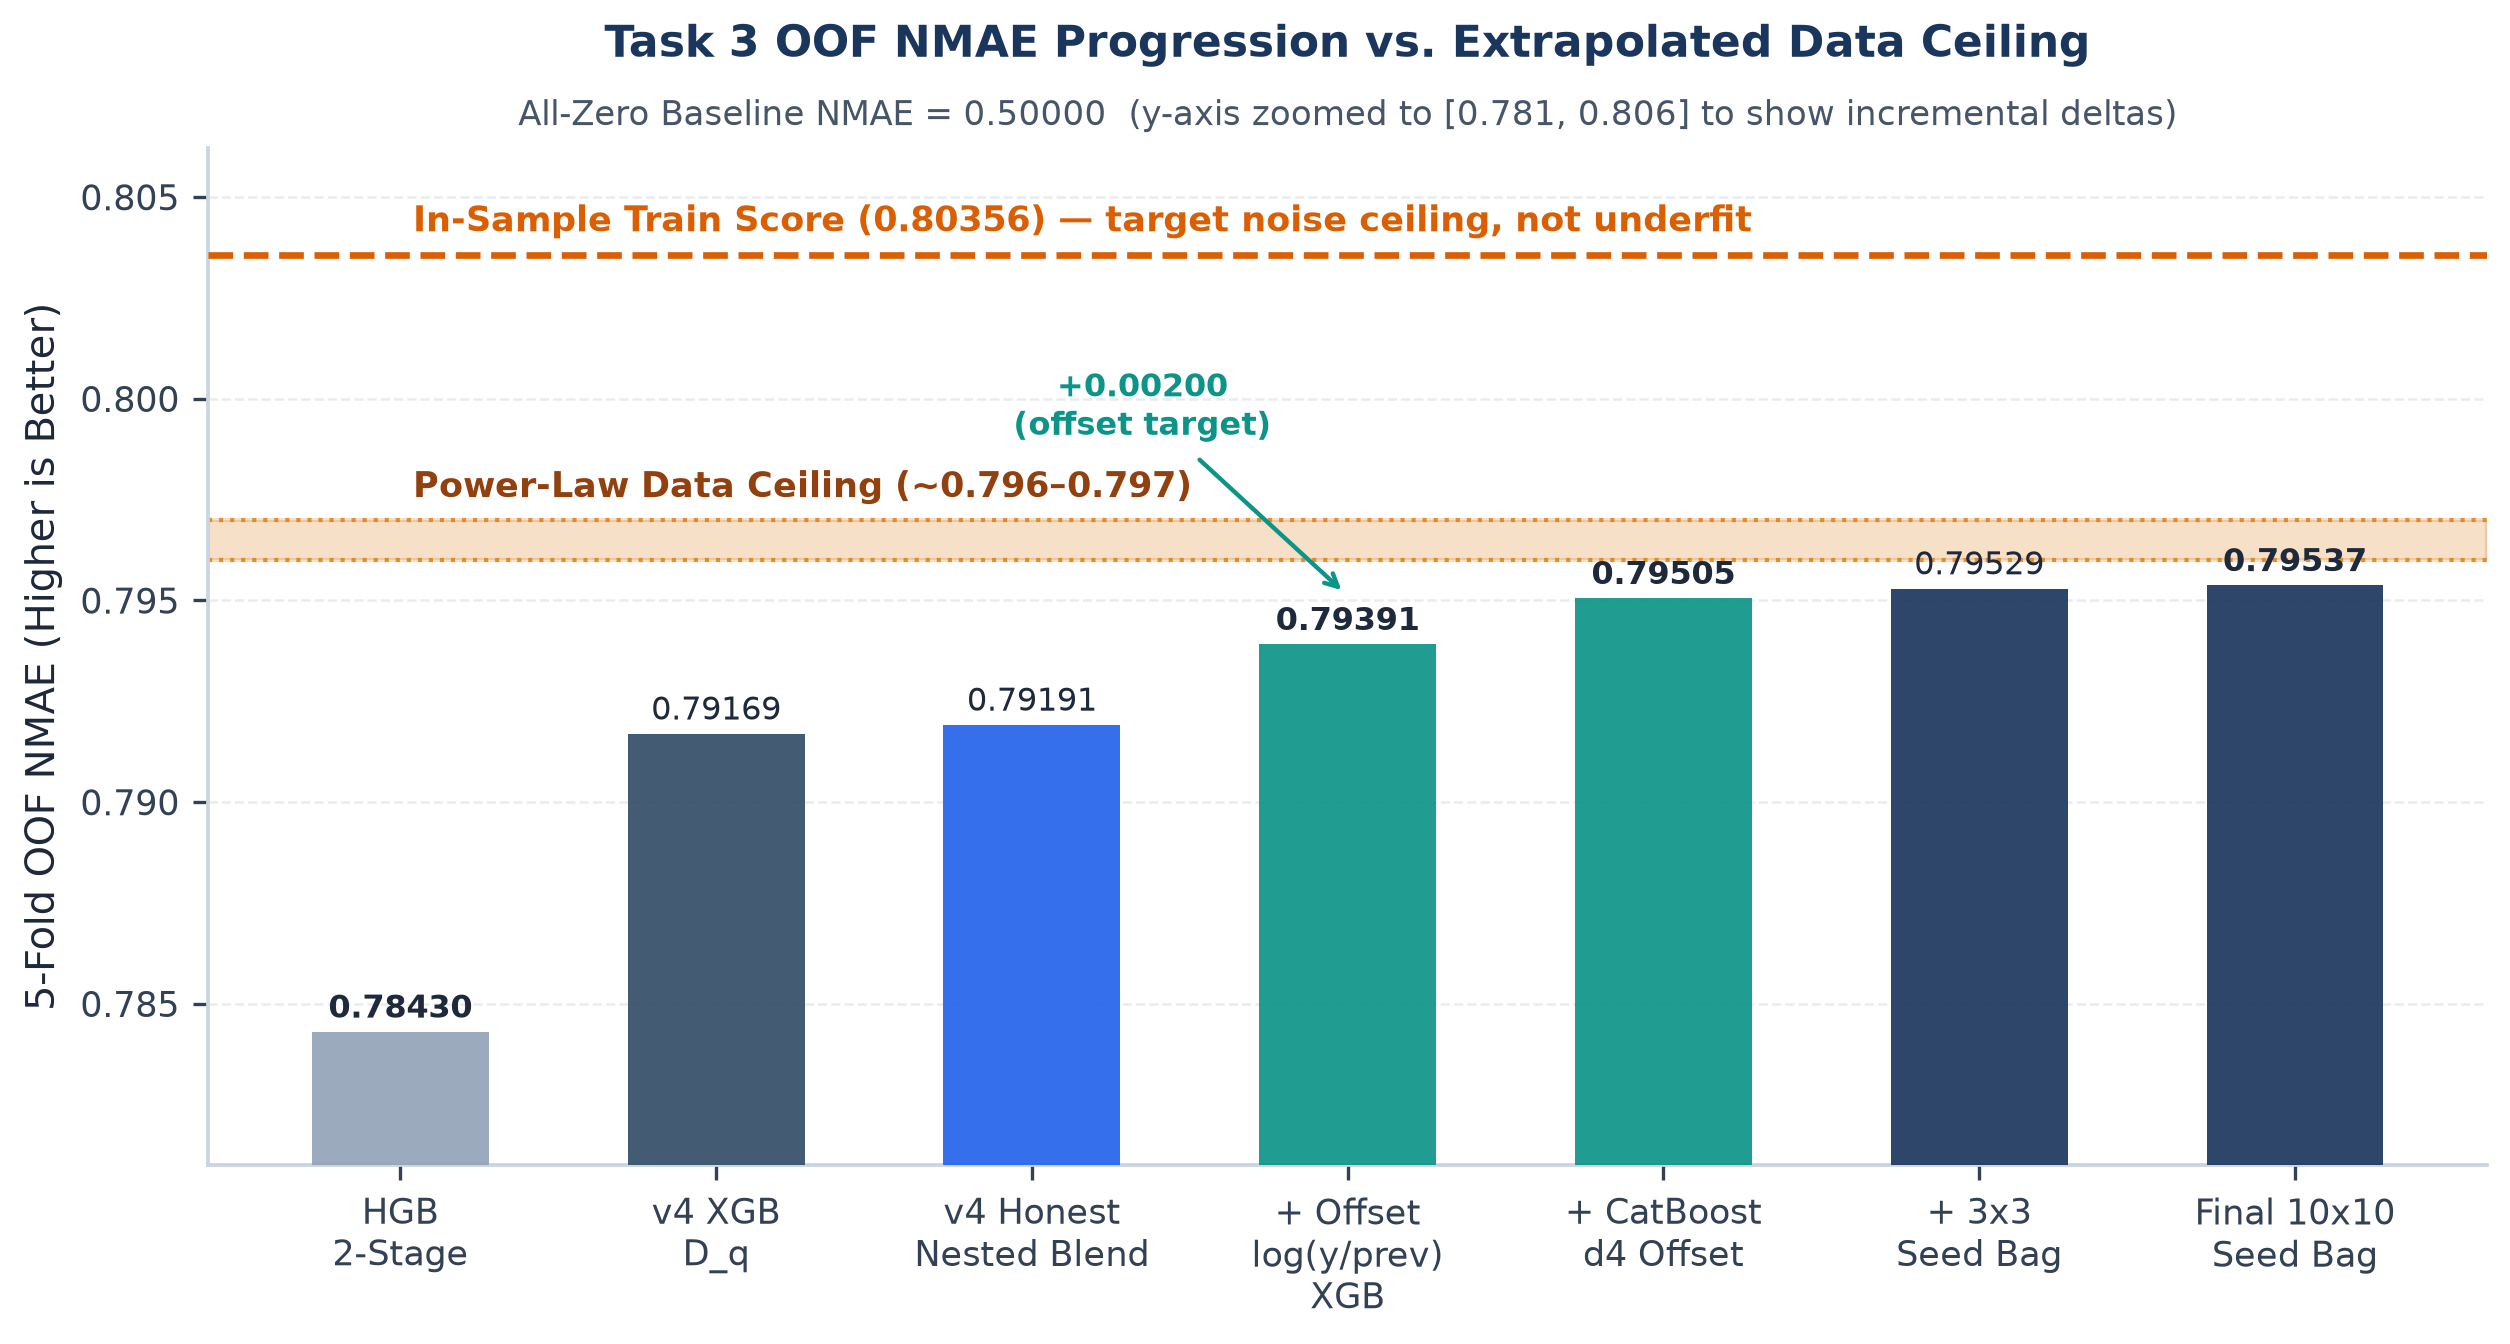
\includegraphics[width=0.95\textwidth]{figures/t3/fig_t3_model_progression_ceiling.png}
    \caption{ความก้าวหน้าของคะแนน 5-Fold OOF NMAE ตั้งแต่ Baseline จนถึง Final 10$\times$10 Seed Bag (\textbf{0.79537}) เทียบกับแถบเพดานข้อมูลจาก Power-Law Learning Curve ($\sim$0.796--0.797) และเส้น In-Sample Train Score (\textbf{0.80356}) ซึ่งยืนยันว่าความคลาดเคลื่อนมาจาก Target Noise มากกว่าความจุของโมเดล}
    \label{fig:t3_progression_ceiling}
\end{figure}

เมื่อนำ \feat{bag\_q10p10} ไปสร้างคำทำนายบนชุดทดสอบ 25,889 แถว (บันทึกในไฟล์ส่งงานสุดท้าย \feat{submissions/FINAL/sub\_v85a\_soup\_trainprior.csv}) การกระจายตัวของค่าทำนายสอดคล้องกับชุดฝึกสอนอย่างแนบแน่น โดยมีอัตราการทำนายศูนย์ \textbf{50.39\%} (เทียบกับ 50.32\% บน OOF และ 48.12\% ค่าจริงใน Train), ค่าเฉลี่ย \textbf{10,429.55 THB} (Train: 10,497.04 THB), ค่ามัธยฐาน \textbf{0.0 THB} (Train: 79.44 THB), เปอร์เซ็นไทล์ที่ 99 \textbf{133,945.49 THB} (Train: 150,032.30 THB) และค่าสูงสุดที่เพดาน \textbf{300,000.0 THB}

\paragraph{การยืนยันสูตรและ OOF-LB Parity ผ่าน Isolated LB Probe}
เพื่อพิสูจน์ว่าสมการ NMAE ที่~\eqref{eq:t3_nmae} ตรงกับตัวชี้วัดบนระบบ Kaggle Public Leaderboard จริง ทีมงานได้ส่ง Probe ทดสอบแบบแยกส่วนโดยนำไฟล์ \feat{probe\_v10e} (คะแนน Public LB 0.67890) มาตั้งค่า Task 3 เป็น 0 ทั้งหมดใน \feat{probe\_v10g} ผลปรากฏว่า Public LB ลดลงเหลือ \textbf{0.61991} คิดเป็นส่วนต่าง \textbf{$\Delta \text{LB} = -0.05899$} เมื่อคำนวณตามน้ำหนักเฉลี่ย 5 ภารกิจ ($w_3 = 0.2$) และคะแนน All-Zero NMAE = 0.50000 จะได้ค่าคาดหมาย $\Delta \text{LB} = 0.2 \times (0.50000 - 0.795) = -0.05900$ ซึ่งตรงกับค่าจริงบน Leaderboard ถึงระดับทศนิยมตำแหน่งที่สี่ ยืนยันทั้งสูตรคำนวณ NMAE และความสอดคล้องสมบูรณ์ระหว่าง OOF CV กับชุดทดสอบจริง

% ----------------------------------------------------------------------
\subsubsection{การวิเคราะห์ Error Budget การทดลองที่ไม่ได้ผล และเพดานของข้อมูล}
\label{subsubsec:t3_error_and_ceiling}

จากสคริปต์วิเคราะห์ความคลาดเคลื่อน \feat{work/insight/c05\_t3\_decomp.py} บน OOF ของโมเดล \feat{bag\_q3p3} (0.79529, $E/Y = 0.2574$) และรูปที่~\ref{fig:t3_whale_budget}(b) สามารถแจกแจงงบประมาณความคลาดเคลื่อนสัมบูรณ์ทั้งหมดออกเป็น 4 แหล่งกำเนิดอย่างครบถ้วน ดังนี้:
\begin{enumerate}
    \item \textbf{สัญญาณรบกวนตัวคูณของผู้จ่ายเงิน (Payer Multiplicative Trapezoid Noise):} เกิดบน \textbf{37,955 แถว} คิดเป็น \textbf{49.0\%} (ค่าจริง 49.03\%, เฉลี่ย 3,630.30 THB/แถว โดย 41.77\% ของ error ทั้งชุดข้อมูลอยู่ภายใน Seg 3) ซึ่งเกิดจากการสุ่มของ Bounded Trapezoid $[0.66\times, 1.38\times]$ ในตัวกำเนิดข้อมูล
    \item \textbf{การโยนเหรียญของผู้ไม่จ่ายเงินที่ถูกทำนาย $> 0$ ($y = 0$ Predicted $> 0$):} เกิดบน \textbf{13,454 แถว} คิดเป็น \textbf{32.9\%} (ค่าจริง 32.87\%, เฉลี่ย 6,864.39 THB/แถว โดย 22.16\% ของ error ทั้งชุดข้อมูลเกิดจาก Whale ที่ไม่จ่ายเงินในเดือนนี้) ซึ่งเป็นความไม่แน่นอนจาก AUC ภายในกลุ่มที่ 0.55--0.63
    \item \textbf{Whale Spikes ที่ถูกสุ่มยอดใหม่:} เกิดบนเพียง \textbf{266 แถว} แต่กินสัดส่วนถึง \textbf{15.4\%} (ค่าจริง 15.43\%, เฉลี่ยสูงถึง 162,993.07 THB/แถว) ของความคลาดเคลื่อนทั้งหมด
    \item \textbf{ผู้จ่ายเงินที่ถูกทำนายเป็น 0 (Payer Predicted 0):} เกิดบน \textbf{15,730 แถว} คิดเป็นเพียง \textbf{2.7\%} (ค่าจริง 2.67\%, เฉลี่ย 477.50 THB/แถว) ส่วนอีก 36,595 แถวที่เหลือคือกลุ่ม $y = 0$ ที่ทำนายได้ 0 อย่างถูกต้อง (ความคลาดเคลื่อนเป็นศูนย์)
\end{enumerate}

\paragraph{เพดานข้อมูล (Oracle Bounds \& Power-Law Ceiling)}
จากการประเมิน Oracle Bounds พบว่าหากตัดเฉพาะ 266 แถวของ Whale Spikes ออก คะแนน OOF จะขยับจาก 0.79529 ไปอยู่ที่ \textbf{0.8135} (0.81349) และหากสมมติให้ทราบตัวตนของผู้ไม่จ่ายเงิน $y = 0$ ล่วงหน้าทั้งหมด (Oracle Zeros โดยใช้โมเดลปริมาณเดิม) คะแนนจะขยับไปที่ \textbf{0.8527} (0.85265) อย่างไรก็ตาม แหล่งความคลาดเคลื่อน 3 อันดับแรก (>97\% ของ error ทั้งหมด) ล้วนมาจากการสุ่มที่คาดการณ์ไม่ได้ของตัวกำเนิดข้อมูล เมื่อทำการทดลอง Learning Curve โดยสุ่มลดจำนวนผู้จ่ายเงินใน training fold เหลือ 25\%, 50\%, 75\% และ 100\% (\feat{R4-03}) คะแนนของ CatBoost \feat{d4} 1 seed อยู่ที่ \textbf{0.79341 / 0.79445 / 0.79501 / 0.79512} ตามลำดับ ซึ่งอัตราการเพิ่มจากการคูณสองของข้อมูลลดลงในอัตรา $\sim 0.6\times$ ต่อรอบ เมื่อใช้กฎกำลัง (Power-Law Extrapolation) ประมาณค่าที่ข้อมูลขนาดอนันต์จะพบเพดานที่ \textbf{$\sim$0.796--0.797} (เช่นเดียวกับ Classifier AUC ที่อิ่มตัวที่ $\sim$0.785 จาก 0.7819 / 0.7830 / 0.7836 / 0.7838) ดังนั้นเป้าหมาย 0.80 (ซึ่งต้องลด $E/Y$ จาก 0.2573 ลงเหลือ 0.2500 หรือ $-2.9\%$) จึงไม่อาจเข้าถึงได้จากฟีเจอร์ชุดนี้ โดยคะแนน In-Sample Train Score เองยังทำได้สูงสุดเพียง \textbf{0.80356}

\paragraph{สรุปการทดลองที่ไม่ได้ผลและถูกปฏิเสธ}
ตารางที่~\ref{tab:t3_failed_exps} รวบรวมกลุ่มการทดลองทั้งหมดที่ให้ผลเป็นกลางหรือแย่ลงเมื่อวัดด้วย Nested/Paired CV อย่างเข้มงวด เพื่อยืนยันว่าไม่มีสัญญาณที่ตกหล่น

\begin{table}[htbp]
\centering
\caption{สรุปผลการทดลองที่ไม่ได้ผลและถูกปฏิเสธในการพัฒนา Task 3 (อ้างอิงเทียบฐานที่ระบุ)}
\label{tab:t3_failed_exps}
\footnotesize
\setlength{\tabcolsep}{4pt}
\begin{tabularx}{\textwidth}{@{}p{3.9cm}p{2.3cm}p{3.0cm}X@{}}
\toprule
\textbf{การทดลอง / แนวคิด} & \textbf{รหัสอ้างอิง} & \textbf{ผล OOF / $\Delta$ เทียบฐาน} & \textbf{ข้อสรุปเชิงวิศวกรรม} \\
\midrule
7 Nested Post-Processing Calibrations & \feat{postproc.py} (\feat{R3-A}--\feat{G}) & $\pm 0.00001$ (0.79527--0.79530 vs 0.79529) & พารามิเตอร์ลู่เข้าหา Identity (\feat{shift}$\approx$0, $\kappa\approx$1.00, \feat{c}=0); กฎ Hurdle Median Calibrated อยู่แล้ว \\
Fitted Linear / Ridge / Hist Offsets & \feat{E08}, \feat{E10}, \feat{E25} & 0.79223 ($-0.0018$), 0.79283 ($-0.0012$), 0.79421 & ความชันที่ประมาณจาก Mean ถูก Whale Spikes บิดเบือน สู้ Unit-Slope \feat{log prev} ไม่ได้ \\
Whale Specialist (Seg 3 เท่านั้น) & \feat{E13} & 0.79148 ($-0.0026$ vs \feat{E07}) & เสียข้อมูลจากกลุ่มอื่นที่มี Step Factors ร่วมกัน \\
Direct Log-Link MAE บน $y$ ดิบ & \feat{E17} & 0.77949 ($-0.0146$ vs \feat{E07}) & Sign-gradient หยุดเร็วที่ $\sim$55 ต้น และเข้าถึงศูนย์แท้จริงไม่ได้ (\feat{frac<1} = 0.1\%) \\
Optuna TPE 31 Trials (ค้นหา Folds 0--1) & \feat{R6-01}--\feat{03} & 0.79509 / 0.79515 (Folds 2--4: $-0.00013$ / $-0.00004$) & ผลบวกบน Folds 0--1 ไม่ถ่ายโอนสู่ Held-out Folds 2--4 (Tuning Fits Noise) \\
Residual Denoising (ตัด 1--10\%, Cauchy) & \feat{R7-01}--\feat{06} & $-0.00001$ ถึง $-0.00031$ vs 0.79512 & Residual กระจายสม่ำเสมอ (\feat{robust sd} 0.17, มีเพียง 0.65\% เกิน 4 sd); Pinball Loss ทน Outlier อยู่แล้ว \\
Unsupervised Outlier Removal (IForest / PCA) & \feat{R8-01}--\feat{04} & IF 1\%: $+0.00013$ (noise); 3/5\%: $-0.00016$/$-0.00024$; Mah: $-0.00008$ & แถวที่แปลกใน Feature Space คือผู้จ่ายจริง การลบออกทำให้สูญเสียข้อมูลฝึกสอน \\
From-Scratch PyTorch MLP (11-Quantile) & \feat{R2-08} & 0.78430 (LAD weight = 0.000 ทุก Fold) & โครงข่ายประสาทรับ Step-Function แนวตั้งได้ด้อยกว่าต้นไม้มาก \\
Nested LAD \& Caruana Blending (12 Families) & \feat{R5-01}--\feat{03} & 0.79526 / 0.79524 / 0.79523 ($-0.00003$ ถึง $-0.00006$) & น้ำหนักแกว่งข้าม Fold ($\text{sd} \le 0.09$); การจูนน้ำหนักแค่ Fit Noise บน OOF \\
Feature Engineering (Fourier, Cadence, Ratio, PCA, Native Cat) & \feat{round12}, \feat{R2-04}, \feat{R8-06}, \feat{c08} & Fourier $-0.00009$ (5/5 แย่), Cadence $-0.00023$, Ratio $-0.00010$, PCA $-0.00007$, Fill $-0.00007$, Native $+0.00007$ & ต้นไม้ดึงข้อมูลจากฟีเจอร์ฐานครบแล้ว ฟีเจอร์เสริมเพิ่มมิติรบกวน \\
Feature-Scale Weighting ($\exp(0.5 \ln \text{prev})$) & \feat{E09} & 0.79263 ($-0.0014$ vs \feat{E07}) & การถ่วงน้ำหนักแถวใหญ่ทำลาย Calibration ของ Quantile Pinball Loss \\
Pooled / Per-Seg Residual Noise Shape & \feat{c09} & 0.79499 / 0.79500 vs 0.79506 & ยืนยันว่ารูปทรงสัญญาณรบกวนคงที่เหมือนกันในทุกผู้จ่าย ไม่ช่วยเพิ่มคะแนน \\
\bottomrule
\end{tabularx}
\end{table}

% ----------------------------------------------------------------------
\subsubsection{การตีความเชิงโดเมนและผลกระทบทางธุรกิจต่อ Karena Thailand}
\label{subsubsec:t3_business_impact}

ผลลัพธ์จากสถาปัตยกรรม Hurdle + Offset CatBoost MultiQuantile ไม่ได้มีคุณค่าเพียงแค่คะแนน OOF NMAE 0.79537 แต่สามารถแปลงเป็นกฎการตัดสินใจเชิงปฏิบัติที่แก้ปัญหาเฉพาะหน้าของ Karena Thailand ได้ทันที 3 ด้าน:

\begin{enumerate}
    \item \textbf{การยุติการแจกโค้ดส่วนลด 50\% ที่สูญเปล่า (Targeted Promo Suppression):} ใช้ผลทำนายจากโมเดลทั้งค่าความน่าจะเป็น $p = P(y > 0)$ และค่า Hurdle Mixture Median $\hat{y}_{\text{med}}$ เพื่อจำแนกผู้เล่นที่ ``จ่ายเงินแน่นอนโดยไม่ต้องกระตุ้น'' โดยเฉพาะกลุ่ม Whale ที่คาดการณ์ $\hat{y}_{\text{med}} > 0$ และมี $p \approx 0.93$ การระงับโค้ดลด 50\% กับผู้เล่นกลุ่มนี้สามารถป้องกันการรั่วไหลของรายได้กว่า \textbf{6 ล้านบาทต่อเดือน} ได้โดยตรง ขณะที่ผู้เล่นซึ่งอยู่บริเวณขอบตัดสินใจ ($p \in [0.40, 0.60]$) หรือมีประวัติการใช้จ่ายจากโปรโมชันสูงเท่านั้นที่จะได้รับข้อเสนอแบบเจาะจง
    \item \textbf{การจัดลำดับความสำคัญของ Ticket สำหรับทีม VIP 20 คน (VIP Ticket Triage):} แทนที่จะจัดคิวตามชั่วโมงการเล่น (\feat{total\_playtime\_hours}) ซึ่งเคยทำให้ทีมเสียเวลาไปกับผู้เล่น 150 รายที่จ่ายรวมกันเพียง 12,000 THB ระบบสามารถจัดลำดับ Ticket ด้วยค่าความน่าจะเป็น \feat{p\_whale} ร่วมกับระดับค่ามัธยฐานเมื่อจ่ายเงิน $Q_{0.50}(y \mid y > 0)$ เพื่อจับคู่ผู้เล่นมูลค่าสูงระดับ 255,000 THB ให้เข้าถึงช่องทางด่วนได้ทันทีและป้องกันการย้ายค่าย
    \item \textbf{การวางแผนกิจกรรมและประมาณการรายได้องค์กร:} สามารถใช้แนวโน้มค่าความน่าจะเป็น $p$ และตัวคูณฤดูกาลรายเดือน (เช่น เดือน 0/11 ที่ $\times 1.26$ และเดือน 5/6 ที่ $\times 1.16$) ช่วยวางตารางปล่อยไอเทม Limited Edition อย่างไรก็ตาม ฝ่ายการเงินต้องแยกใช้ตัวพยากรณ์คนละตัวกับการคัดกรองโปรโมชันตามคำเตือนเชิงเทคนิคด้านล่าง
\end{enumerate}

\begin{warningbox}[ข้อควรระวังในการนำไปใช้งาน: Conditional Median vs. Expected Revenue Aggregation]
แม้ค่า \textbf{Conditional Mixture Median} ($\hat{y}_{\text{med}} = 0$ เมื่อ $p \le 0.5$ และ $Q_{1 - 1/(2p)}$ เมื่อ $p > 0.5$) จะเป็นคำตอบที่ดีที่สุดทางคณิตศาสตร์สำหรับลด MAE และเหมาะอย่างยิ่งสำหรับการคัดกรองไม่ให้แจกส่วนลดพร่ำเพรื่อ \textbf{แต่ฝ่ายการเงินห้ามนำค่า Mixture Median ของผู้เล่นทุกคนมาบวกรวมกันเพื่อพยากรณ์รายได้รวมรายไตรมาสของบริษัทโดยเด็ดขาด}

เหตุผลทางคณิตศาสตร์คือ สำหรับการแจกแจงแบบ Zero-Inflated และเบ้ขวาอย่างรุนแรง ค่ามัธยฐานมักต่ำกว่าค่าคาดหมายมาก โดยเฉพาะผู้เล่นกลุ่ม Casual (\feat{segment} = 0) ซึ่งมี $p \le 0.5$ เกือบทั้งหมด ทำให้ค่าเฉลี่ยของ OOF Mixture Median ในกลุ่มนี้ตกต่ำเหลือเพียง \textbf{4.81 THB} เทียบกับรายได้เฉลี่ยจริง \textbf{73.96 THB} (หายไปถึง \textbf{-93.5\%}) แม้ในการทดสอบ OOF รวมทุกกลุ่ม ผลรวมของ Mixture Median (\textbf{10,514.78 THB}/ราย) จะใกล้เคียงค่าเฉลี่ยจริง (\textbf{10,497.04 THB}/ราย, ต่างกัน $+0.17\%$) จากการหักล้างกันโดยบังเอิญระหว่างกลุ่ม Seg 0/3 ที่ต่ำกว่าจริงกับ Seg 1/2 ที่สูงกว่าเล็กน้อย แต่ความสมดุลดังกล่าวจะพังทลายทันทีเมื่อโครงสร้างฐานผู้เล่นเปลี่ยนไปสู่กลุ่มใหม่ที่มี $p \le 0.5$ เป็นหลัก (เช่น Cohort ผู้เล่นใหม่ ซึ่งผลรวม Median จะทำนายรายได้เป็น 0 บาท)

ดังนั้น ตามหลัก \textbf{Linearity of Expectation} ($\mathbb{E}[\sum_i Y_i] = \sum_i \mathbb{E}[Y_i \mid \mathbf{x}_i]$) ระบบพยากรณ์งบประมาณองค์กรจึงต้องคำนวณผลรวมของ \textbf{ค่าคาดหมายแบบมีเงื่อนไข} $\sum_{i=1}^{N} \hat{p}_i \cdot \widehat{\mathbb{E}}[Y_i \mid Y_i > 0, \mathbf{x}_i]$ จากโมเดลส่วนคาดหมายในสเกลบาท (หรือการอินทิเกรตตลอดการแจกแจงควอนไทล์ของ \feat{bag\_q10p10}) เพื่อลดความคลาดเคลื่อนการประมาณการรายได้ระดับองค์กรจาก 35--40\% ให้ได้อย่างยั่งยืนและไม่เกิดอคติเชิงระบบ
\end{warningbox}
